% =====================================================================
%  It's the Labels, Not the Model
%  Skeleton -- ROADMAP Phase 5. Section map follows PAPER_OUTLINE.md §3.
%
%  Compiles as-is with pdflatex + a standard TeX Live. To move to the
%  CVPR workshop template, replace the two lines marked TEMPLATE below
%  with \documentclass[10pt,twocolumn,letterpaper]{article} + \usepackage{cvpr}
%  (or IEEEtran for GRSL). Nothing else in this file assumes a class.
%
%  ⚠️ EVERY NUMBER COMES FROM numbers.tex. Do not type a figure inline --
%  if it is not a macro there, it has no citation and does not belong.
% =====================================================================
\documentclass[10pt,a4paper]{article}                        % TEMPLATE
\usepackage[margin=2.2cm]{geometry}                          % TEMPLATE

\usepackage[T1]{fontenc}
\usepackage[utf8]{inputenc}
\usepackage{graphicx}
\usepackage{booktabs}
\usepackage{amsmath,amssymb}
\usepackage{multirow}
\usepackage{xcolor}
\usepackage{siunitx}
\sisetup{detect-weight=true, detect-family=true}
\usepackage[hidelinks]{hyperref}

\graphicspath{{../docs/}}
% =====================================================================
%  Every load-bearing number in the paper, defined ONCE.
%
%  WHY THIS FILE EXISTS. This project has caught five silent errors, and
%  the cheapest class of error left is a number that is right in the
%  results table and stale in the abstract. Macros make that impossible:
%  change it here and it changes everywhere, or it changes nowhere.
%
%  Each macro carries the file and section it came from. If a macro has
%  no citation it is not allowed in the paper.
% =====================================================================

% ---- baselines ------------------------------------------------------
\newcommand{\loveBase}{47.38}        % WEEK1 §5   reproduced, full val
\newcommand{\lovePub}{47.4}          % SegEarth-OV3, Table 1
\newcommand{\loveInstr}{47.37}       % WEEK1 §5   instrumented recompute (the gate)
\newcommand{\oemBase}{44.19}         % WEEK3 §7   384 of 500 val tiles
\newcommand{\oemPub}{42.9}           % SegEarth-OV3, published
\newcommand{\loveTiles}{1669}
\newcommand{\oemTiles}{384}

% ---- the residual ---------------------------------------------------
\newcommand{\discardPct}{29.68\%}    % WEEK1 §7.1
\newcommand{\discardPx}{323{,}184{,}908}
\newcommand{\discardOEM}{3.78\%}     % WEEK3 §7
\newcommand{\discardRatio}{3:1}      % WEEK1 §7.6  discard vs confusion
\newcommand{\mechA}{94.0\%}          % WEEK1 §7.7  below tau
\newcommand{\mechB}{6.0\%}           % WEEK1 §7.7  background won the argmax
\newcommand{\mechBpx}{19{,}378{,}177}
\newcommand{\mechBtiles}{24}
\newcommand{\mechBpots}{1.25\%}    % POTSDAM, reachability.py 4 Sep: argmax loss
\newcommand{\cnOemFloor}{0.1042}    % CONINFER_RESULTS: their OEM cache conf floor
\newcommand{\cnOemTau}{0.1}         % their published prob_thd on OpenEarthMap


% ---- the mechanism --------------------------------------------------
\newcommand{\bgShareLove}{36.1\%}    % WEEK3 §7
\newcommand{\bgShareOEM}{0.84\%}
\newcommand{\aucLove}{0.622}         % best of nine signals
\newcommand{\aucOEM}{0.913}          % conf2
\newcommand{\aucFloor}{0.53}         % empirical, size-stratified
\newcommand{\presCorrLove}{-0.750}
\newcommand{\presCorrOEM}{+0.094}
\newcommand{\catTilesLove}{198}
\newcommand{\catTilesOEM}{0}

% ---- refuted interventions -----------------------------------------
\newcommand{\tauCost}{-5.54}         % WEEK1 §7.2  tau 0.5 -> 0.1
\newcommand{\tauRatio}{1.73}         % WEEK1 §8.2  wrong per right
\newcommand{\presCost}{-11.97}       % WEEK1 §9.2b
\newcommand{\recoverLove}{+0.04}     % WEEK3 §8
\newcommand{\recoverOEM}{+2.28}      % WEEK3 §8   -- NEVER without \oemBgGain
\newcommand{\oemBgGain}{+22.67}      % WEEK3 §8.1
\newcommand{\oemRealLoss}{-2.11}     % WEEK3 §8.1
\newcommand{\oemBuildLoss}{-3.75}    % WEEK3 §8.1
\newcommand{\priorGain}{+0.2}        % WEEK3 §6   over a neighbour vote
\newcommand{\priorOracle}{+0.3}      % WEEK3 §6   with a PERFECT matrix

% ---- atomisation ----------------------------------------------------
\newcommand{\ceilCC}{72.8\%}         % WEEK3 §4
\newcommand{\ceilSLIC}{92.8\%}
\newcommand{\ceilSLICoem}{82.9\%}

% ---- the method -----------------------------------------------------
\newcommand{\methodGain}{+1.18}      % WEEK3 §9b  5-fold mean
\newcommand{\methodSD}{0.45}
\newcommand{\methodWorst}{+0.80}
\newcommand{\methodLand}{+8.30}      % 5-fold, six real classes
\newcommand{\methodBg}{-0.01}
\newcommand{\methodWater}{+6.78}
\newcommand{\methodWaterTau}{0.195}
\newcommand{\oracleBound}{+1.46}     % WEEK3 §9a  per-class oracle
\newcommand{\oracleShare}{81\%}
\newcommand{\globalOracle}{+0.04}    % WEEK3 §9a  best GLOBAL tau
\newcommand{\calibTiles}{200}        % WEEK3 §9b  every draw positive
\newcommand{\trainToVal}{-0.12}      % WEEK3 §9b  scope limit

% ---- end-to-end verification ---------------------------------------
\newcommand{\eeBase}{47.16}          % WEEK3 §9c  held-out tiles
\newcommand{\eeFit}{48.35}
\newcommand{\eeTiles}{1469}
\newcommand{\eeSpread}{0.175--0.675}

% ---- the label-free bound ------------------------------------------
\newcommand{\proxyBest}{+0.42}       % WEEK3 §9d  presence, best of eight
\newcommand{\proxyCtrl}{+0.58}       % random-control p95
\newcommand{\proxyConfRho}{+0.943}   % mean_conf vs precision
\newcommand{\proxyConfP}{0.017}
\newcommand{\proxyHeadRho}{+0.886}   % sem_inst_agree vs precision
\newcommand{\proxyHeadP}{0.033}
\newcommand{\proxyTauRho}{-0.429}    % precision vs ORACLE TAU -- the broken link
\newcommand{\proxyTauP}{0.419}
\newcommand{\nAttempts}{eleven}      % 3 threshold rules + 8 proxies

% ---- the co-occurrence prior ---------------------------------------
\newcommand{\pmiSignal}{0.574}       % ANALYSIS §4, corrected marginal
\newcommand{\pmiFloor}{0.003}
\newcommand{\pmiRatio}{216}
\newcommand{\rhoMined}{+0.757}       % WEEK3 §5  gate 1
\newcommand{\rhoCirc}{-0.257}        % circularity, retired

% ---- the confound stratification (WEEK3 §7a) -----------------------
\newcommand{\SHAREr}{42.9\%}       % LoveDA rural, catch-all share of GT
\newcommand{\SHAREu}{26.0\%}       % LoveDA urban
\newcommand{\CONFr}{25.5\%}        % rural confusability, measured
\newcommand{\CONFu}{43.3\%}        % urban -- the LOWER-share stratum is more confusable
\newcommand{\AUCr}{0.524}          % rural detection AUC (conf)
\newcommand{\AUCu}{0.730}          % urban

% ---- WEEK3_RESULTS.md 9e: per-class tau across LoveDA's domains -------------
\newcommand{\DOMr}{+2.77}          % rural within-domain gain, 5-fold
\newcommand{\DOMrsd}{0.92}
\newcommand{\DOMu}{+0.10}          % urban -- NOT distinguishable from zero (2/5 folds)
\newcommand{\DOMusd}{0.39}
\newcommand{\DOMrreal}{+18.61}     % rural, real classes aggregate
\newcommand{\DOMureal}{+4.18}      % urban, real classes aggregate -- land cover DOES gain
\newcommand{\DOMubg}{-3.51}        % urban catch-all pays for it: (4.18-3.51)/7 = +0.10
\newcommand{\DOMtaudiff}{0.227}    % mean |tau difference| between the domains
\newcommand{\DOMtaumax}{0.500}     % max, on `road' (0.725 rural vs 0.225 urban)
\newcommand{\DOMxr}{-0.40}         % mismatched -> rural, BELOW the published tau
\newcommand{\DOMxu}{-1.11}         % mismatched -> urban, BELOW the published tau
\newcommand{\DOMmr}{+2.32}         % matched -> rural, same 200-tile budget
\newcommand{\DOMmu}{+0.02}         % matched -> urban
\newcommand{\DOMpr}{+0.77}         % pooled -> rural: keeps a third of matched
\newcommand{\DOMpu}{-0.32}         % pooled -> urban

% ---- WEEK3_RESULTS.md 7b: the vocabulary intervention ----------------------
% det = max(AUC, 1-AUC). AUC is symmetric, so a raw AUC of 0.208 is a detector
% of strength 0.792 inverted, NOT an absent signal. Never quote raw AUC here.
\newcommand{\ivA}{0.794}           % A0, published vocabulary, det(conf)
\newcommand{\ivAtwo}{0.913}        % A0, det(conf2)
\newcommand{\ivShareA}{0.84\%}     % catch-all share, published
\newcommand{\ivShareD}{58.20\%}    % catch-all share, largest dose
\newcommand{\ivB}{0.582}           % faithful dose arm, det(conf)
\newcommand{\ivBtwo}{0.590}        % faithful dose arm, det(conf2)
\newcommand{\ivD}{0.710}           % arity-matched control, det(conf)
\newcommand{\ivDtwo}{0.855}        % arity-matched control, det(conf2)
\newcommand{\ivRatio}{2.5$\times$} % dose effect / control effect, conf
\newcommand{\ivRatioTwo}{5.6$\times$}  % ... conf2
\newcommand{\ivRatioWorst}{3.1$\times$} % conf2 vs the WORST control, not the matched one
\newcommand{\ivArms}{13}           % arms, all reading one cached score stack

% ---- WEEK3_RESULTS.md 7c: the reverse arm, and what bounds the mechanism ----
\newcommand{\ivRev}{0.540}         % LoveDA, catch-all removed from the VOCABULARY
\newcommand{\ivRevBase}{0.592}     % LoveDA A0 -- vocabulary change alone does nothing
\newcommand{\ivVocabMax}{0.052}    % largest move by ANY arm that leaves GT share alone
\newcommand{\ivSatShare}{35\%}     % above this, four points sit in one band
\newcommand{\ivSatLo}{0.58}
\newcommand{\ivSatHi}{0.64}

% ---- WEEK3_RESULTS.md 9f: no label-free rule for WHEN calibration pays ------
\newcommand{\crProxyRho}{+0.885}   % label-free catch-all fraction vs labelled discard, LoveDA
\newcommand{\crProxyRhoOEM}{+0.924}
\newcommand{\crLow}{$+2.13 \pm 0.18$}   % LEAST-residual stratum -- the most reliable gain
\newcommand{\crHigh}{$+3.22 \pm 3.15$}  % most-residual stratum -- worst fold -1.22
\newcommand{\crRho}{+0.400}        % LoveDA, over 4 strata
\newcommand{\crRhoOEM}{-0.500}     % OEM -- opposite sign, nothing replicates

% ---- WEEK3_RESULTS.md 9g: what the domain gap is made of --------------------
\newcommand{\cpWater}{48\%}        % water's share of the rural/urban gap
\newcommand{\cpForest}{37\%}       % forest's share
\newcommand{\cpTop}{85\%}          % the two together
\newcommand{\cpGapRho}{+0.713}     % P-R gap vs per-class delta IoU, 12 cells
\newcommand{\cpGapP}{0.013}        % permutation p
\newcommand{\cpPrecRho}{+0.168}    % precision ALONE -- explains nothing
\newcommand{\cpPrecP}{0.60}

% ---- WEEK3_RESULTS.md 9h: both metrics ------------------------------------
% ⚠️ ALWAYS the per-class MEAN (= catch-all-excluded mIoU), never the aggregate
% sum. Sections 9b/9e quote sums; +8.30 aggregate IS +1.38 here. Mixing them puts
% two numbers 6x apart in units next to each other.
\newcommand{\mrLoveFull}{+1.16}    % LoveDA, full mIoU, 5-fold held out
\newcommand{\mrLoveReal}{+1.36}    % LoveDA, catch-all-excluded mIoU
\newcommand{\mrLoveBg}{-0.02}
\newcommand{\mrOemFull}{+0.30}     % OEM, full mIoU -- looks flat
\newcommand{\mrOemReal}{+1.75}     % OEM, catch-all-excluded -- LARGER than LoveDA
\newcommand{\mrOemBg}{-11.30}
\newcommand{\mrOemLand}{+1.56}     % the real classes' contribution to full mIoU
\newcommand{\mrOemBgC}{-1.26}      % background's contribution: cancels it
\newcommand{\mrOemDistort}{3.38}   % OEM's baseline headline depression
\newcommand{\mrLoveLever}{14.3\%}  % 1/N -- the catch-all's share of the metric
\newcommand{\mrOemLever}{11.1\%}
\newcommand{\mrOemBgIoU}{17.13}
\newcommand{\methodLandMean}{+1.38}  % 9b's +8.30 aggregate, in mIoU units

% ---- CONINFER_RESULTS.md 7.1a: per-class tau on a CLIP backbone -------------
% ⚠️ Deltas measured on OUR reproduction (36.99), not their published 39.33. A
% delta is robust to a constant offset, but the text must say so.
\newcommand{\cnPub}{39.33}         % ConInfer's published LoveDA mIoU
\newcommand{\cnRepro}{36.99}       % our reproduction -- gap -2.34, full split
\newcommand{\cnGap}{2.34}          % CONINFER_RESULTS: repro below published
\newcommand{\cnTau}{0.8}           % THEIR published LoveDA threshold
\newcommand{\cnBase}{37.00}        % held-out baseline at their tau
\newcommand{\cnFit}{39.52}         % held out, per-class tau
\newcommand{\cnFull}{+2.52}
\newcommand{\cnReal}{+1.94}        % catch-all-excluded -- above SAM 3's +1.36
\newcommand{\cnBg}{+6.01}
\newcommand{\cnCV}{+2.51}          % five-fold mean
\newcommand{\cnCVsd}{0.34}
\newcommand{\cnWorst}{+2.22}       % every fold positive
\newcommand{\cnCalib}{25}          % tiles for a reliable gain -- 8x cheaper here
% ConInfer on OpenEarthMap: the transfer does NOT hold there, and why
\newcommand{\cnOemCV}{-0.39}       % five-fold, sd 1.28, 1/5 folds positive
\newcommand{\cnOemCVsd}{1.28}
\newcommand{\cnOemFull}{-0.09}
\newcommand{\cnOemReal}{+1.27}     % land cover DOES improve
\newcommand{\cnOemBg}{-10.94}      % catch-all sacrificed: 17.00 -> 6.06
\newcommand{\cnOemBgAfter}{6.06}
\newcommand{\mrOemBgAfter}{5.83}   % SAM 3 drives it to almost the same value

% ---- third dataset + the supervised-gap framing ----------------------------
\newcommand{\potsBase}{57.83}      % our Potsdam reproduction
\newcommand{\potsPub}{57.8}        % SegEarth-OV3 published -- matches to 0.03
\newcommand{\potsTiles}{2016}      % val tiles, 512^2, stride 512
% ⭐ The oracle is a fully supervised SegFormer-b0 with full training data,
% reported in SegEarth-OV3's own Table 2. Framing the gain as a share of the
% supervised gap is far more legible than a raw delta.
\newcommand{\oracleSup}{50.0}      % LoveDA, fully supervised
\newcommand{\gapClosed}{44\%}      % (48.53-47.37)/(50.0-47.37)

% ---- POTSDAM_RESULTS.md: the third dataset ---------------------------------
\newcommand{\potsShare}{4.29\%}    % `clutter` share of GT -- PRE-REGISTERED
\newcommand{\potsDiscard}{4.68\%}  % measured; committed bracket was 3.78-10.88%
\newcommand{\potsPoint}{4.5\%}     % the committed point estimate
\newcommand{\potsAuc}{0.578}       % best CACHED signal -- prediction was >0.622
% ⚠️ \aucLove is 0.622, LoveDA's best signal INCLUDING texture. For a like-for-like
% comparison with Potsdam (cached signals only) the LoveDA figure is 0.582.
\newcommand{\aucLoveCached}{0.582}
\newcommand{\aucOemCached}{0.794}
\newcommand{\potsReal}{+1.04}      % catch-all-excluded mIoU
\newcommand{\potsFull}{+0.59}      % five-fold full mIoU
\newcommand{\potsFullSd}{0.50}     % spread covers zero -- marginal, say so
\newcommand{\potsDistort}{8.18}    % clutter depresses the headline by this much

% ---------------------------------------------------------------------
%  THE SECOND LEVER: per-class scaling before the argmax.
%  ARGMAX_SCALING_RESULTS.md. All five-fold figures come from one script
%  (argmax_reorder.py) so the substitution table compares like with like.
% ---------------------------------------------------------------------
\newcommand{\scLove}{+1.16}          % LoveDA  C-B, 5-fold
\newcommand{\scLoveSD}{0.19}
\newcommand{\scLoveExcl}{+1.36}      % catch-all-excluded
\newcommand{\scLoveBg}{-0.03}
\newcommand{\scPots}{+4.86}          % Potsdam C-B, 5-fold
\newcommand{\scPotsSD}{0.35}
\newcommand{\scCI}{-0.10}            % ConInfer C-B, 5-fold
\newcommand{\scCISD}{0.14}
\newcommand{\scCIfolds}{1 of 5}
% the substitution table -- all five-fold, same script
\newcommand{\subCItau}{+2.51}
\newcommand{\subLovetau}{+1.16}
\newcommand{\subPotstau}{+0.59}
% end-to-end verification
\newcommand{\eeScaleLove}{+1.34}     % measured increment, LoveDA
\newcommand{\eeScaleLovePred}{+1.31}
\newcommand{\eePotsA}{57.60}
\newcommand{\eePotsB}{58.35}
\newcommand{\eePotsC}{63.27}
\newcommand{\eePotsScale}{+4.92}
\newcommand{\eePotsTotal}{+5.67}
\newcommand{\eePotsMiss}{0.05}       % worst rung miss vs prediction
\newcommand{\eePotsClassMiss}{0.23}  % worst per-class miss
% the tree case
\newcommand{\treeGap}{+54.7}
\newcommand{\treeP}{93.34}
\newcommand{\treeR}{38.63}
\newcommand{\treeTau}{+0.32}         % what per-class tau moved it
\newcommand{\treeScale}{+21.17}      % what the scale moved it, measured
\newcommand{\treeW}{3.73}
\newcommand{\scCalibPots}{100}
\newcommand{\confusionShare}{9.9\%}   % WEEK1 7.6: real-class confusion, LoveDA
\newcommand{\scSpread}{15\%}   % worst real-class fold spread, Potsdam (road)

% ---- the qualitative figure (scripts/fig_qualitative.py, Potsdam val) --------
% Row 4 is a tile where the method LOSES. It is in the figure deliberately: the
% five-fold Potsdam gain \scPots{} is an AVERAGE and four wins would misstate it.
\newcommand{\qualLoss}{7.72}         % 2_13_1024_0_1536_512, full mIoU 41.04->33.32
\newcommand{\qualLossRight}{26.1\%}  % of its changed pixels that became correct

% ---- the open-vocabulary run on Indian UAV imagery (scripts/fig_vocabulary.py)
% ⛔ NO GROUND TRUTH. These are per-class PIXEL SHARES with nodata excluded, not
% accuracy. Nothing derived from them may be phrased as a correctness claim.
\newcommand{\indTiles}{25}           % tiles cut from 5 OpenAerialMap scenes
\newcommand{\indScenes}{5}
\newcommand{\indGSD}{4--5\,cm}
\newcommand{\indFloodA}{78.6}        % `water` under the settlement vocabulary
\newcommand{\indFloodB}{79.1}        % `flood water` under the Indian one
\newcommand{\indBldgA}{18.2}         % `concrete roof`
\newcommand{\indBldgB}{18.3}         % `building`
\newcommand{\indVegA}{100.0}         % solar-farm tile collapses to ONE class
\newcommand{\indSolarB}{4.6}         % ⚠️ PARTIAL -- far below the panels' extent

% the tree case, absolute -- ARGMAX_SCALING_RESULTS.md, measured by eval.py on
% 1816 held-out Potsdam tiles. \treeScale is their difference.
\newcommand{\treeIoUa}{37.92}
\newcommand{\treeIoUb}{59.09}

% ---- combined totals, for the review presentation --------------------------
% Both levers together. LoveDA = \methodGain + \scLove ; Potsdam = eePotsC-eePotsA,
% measured end-to-end by eval.py, not summed from folds.
\newcommand{\loveTotal}{+2.32}       % 1.18 (tau) + 1.16 (scale), 5-fold
\newcommand{\potsTotal}{+5.67}       % 57.60 -> 63.27, eval.py, 1816 held-out tiles
\newcommand{\potsExcl}{+6.00}        % Potsdam catch-all-excluded, 5-fold

% ---- how much of the residual comes back -----------------------------------
% @DISCARD_AFTER_RESULTS.md, 12 Sep. scripts/discard_after.py, LoveDA full 1669
% tiles, 5-fold held out. The accounting identity
%   discard_A - discard_X == recovered - newly discarded
% is verified as exact integers on every run. Rates from a 40k px/tile
% subsample (42.9M real-class px scored); measure_discard_rate.py owns the
% absolutes at the published tau.
\newcommand{\raDiscA}{29.25\%}       % rung A, published tau
\newcommand{\raDiscB}{26.77\%}       % rung B, per-class tau
\newcommand{\raDiscC}{25.01\%}       % rung C, + per-class scale
\newcommand{\raDrop}{4.24}           % points, A -> C
\newcommand{\raRecov}{4.65\%}        % recovered vs A, rung C
\newcommand{\raNew}{0.40\%}          % newly discarded, rung C -- NEVER quote
                                     % \raRecov without this one (WEEK1 8.2)
\newcommand{\raCorrect}{79.2\%}      % of recovered, landing on the right class
\newcommand{\raWPR}{0.26}            % wrong per right, ours
\newcommand{\raTauCorrect}{36.6\%}   % of recovered, tau->0.1 = 1/(1+\tauRatio)
\newcommand{\raFactor}{6.6}          % \tauRatio / \raWPR
% per class, rung C. The four whose tau moved DOWN recover well; the two whose
% tau moved UP recover almost nothing and get it wrong -- by design.
\newcommand{\raWaterA}{31.9\%}
\newcommand{\raWaterC}{18.6\%}
\newcommand{\raWaterOk}{95.0\%}
\newcommand{\raRoadDelta}{+0.1}      % road DISCARDS MORE, deliberately

% ---- separability of the real objective ------------------------------------
% @SEPARABILITY_RESULTS.md. For a FIXED argmax a pixel predicted c either clears
% tau_c or becomes the catch-all -- never another real class -- so TP/FP/FN for
% class c depend on tau_c alone and the `real' objective is a sum of
% single-variable terms. Measured at exactly 0 on every class sweep.
\newcommand{\sepExact}{0.000000}     % max |delta tau| over all sweeps
\newcommand{\sepSweeps}{19}          % class-sweeps, LoveDA + Potsdam + OEM
\newcommand{\sepCostA}{$N\times201$} % cost of exact coordinate ascent
\newcommand{\sepCostB}{$201^{N}$}    % cost of the naive joint search
\newcommand{\sepAllMax}{0.0050}      % Potsdam, --objective all: it does NOT hold

% ---- how much of the oracle the fit captures -------------------------------
% Held-out real-class mIoU. Put this in limitations: it is a measured bound on
% the method, and naming it is stronger than letting a reader compute it.
\newcommand{\capLove}{83\%}
\newcommand{\capPots}{73\%}
\newcommand{\capOEM}{11\%}
\newcommand{\capOemWaterFit}{0.710}   % OEM water, fitted
\newcommand{\capOemWaterOra}{0.240}   % OEM water, oracle
\newcommand{\capOemWaterA}{69.18}     % its IoU at the oracle threshold
\newcommand{\capOemWaterB}{55.02}     % ... and at the fitted one

% ---- the one-standard-error rule: tested, and worse than what we deploy -----
\newcommand{\seLove}{+0.76}          % vs deployed +1.23
\newcommand{\sePots}{+0.55}          % vs deployed +0.90
\newcommand{\seOEM}{+0.54}           % vs deployed +0.28
\newcommand{\seMean}{-0.19}          % mean delta vs the deployed rule

% ---- which classes to calibrate: closed by an UPPER BOUND ------------------
% scripts/freeze_selection.py, LoveDA 1669 tiles, 5-fold held out.
\newcommand{\frzOracle}{+0.08}       % choosing on the EVALUATION fold
\newcommand{\frzCv}{-0.07}           % honest inner-CV selection

% ---- the five levers, one protocol ----------------------------------------
% Levers 1-2 reshape the DECISION and work; 3-5 are reported as bounded
% negatives. Every one was pre-registered.
\newcommand{\lvThreePots}{+0.04}     % head fusion, Potsdam
\newcommand{\lvThreeLove}{+0.22}     % head fusion, LoveDA
\newcommand{\lvFour}{+0.16}          % per-class presence weight, LoveDA
\newcommand{\lvFive}{-0.07}          % per-class bias (vector scaling), LoveDA
\newcommand{\lvFiveSD}{0.18}
\newcommand{\lvRhoCar}{2.33}         % Potsdam car -> instance head
\newcommand{\lvRhoBuild}{0.53}       % Potsdam building -> semantic head
\newcommand{\lvGammaRho}{+0.886}     % Spearman(median S_pres, gamma), p=0.017
\newcommand{\lvGammaP}{0.017}

% ---- sliding-window inference: tested, and it costs -------------------------
% @SLIDING_WINDOW_RESULTS.md. slide_crop=512, stride=341, LoveDA val 1669 tiles.
% SAM 3 resizes input to 1008^2, so 512^2 crops are UPSAMPLED ~2x -- the
% configuration the rest of this literature uses and SegEarth-OV3 does not.
% Precision RISES and recall COLLAPSES, which is a tighter gate rather than
% sharper features: S_pres is computed per view, so a class absent from a crop
% is vetoed there.
\newcommand{\swMIoU}{43.53}          % vs the published single-view 47.38
\newcommand{\swDelta}{-3.85}
\newcommand{\swPrec}{+1.1}           % mPrecision, single-view -> sliding-window
\newcommand{\swRec}{-4.7}            % mRecall
\newcommand{\swWater}{-14.28}        % water IoU, over half the total loss
\newcommand{\swWaterRec}{-16.1}      % water recall
\newcommand{\swBgRec}{+12.9}         % background recall: the catch-all absorbs MORE
\newcommand{\swCrop}{$512$}

% ---- and the gate was MITIGATING the loss, not causing it ------------------
% @SLIDING_WINDOW_RESULTS.md 2a. Loosening the presence gate under sliding
% window costs MORE, and precision collapses while recall barely moves -- so the
% per-crop veto was suppressing false positives, not valid predictions.
\newcommand{\swMax}{39.86}           % gate = max presence over crops
\newcommand{\swGlobal}{39.05}        % gate = one whole-image forward
\newcommand{\swMaxDelta}{-3.67}      % vs the per-crop gate
\newcommand{\swPrecDrop}{68.1 \rightarrow 58.2 \rightarrow 56.7}
\newcommand{\swBuildPrec}{77.0 \rightarrow 49.4}

% ---- dihedral test-time augmentation --------------------------------------
% @TTA_RESULTS.md. Average the score stacks over flipped/rotated views of the
% WHOLE image -- unlike crops, the field of view and therefore the presence
% semantics are identical across views, which is why this works where sliding
% window did not. Aerial imagery has no canonical orientation, so the argument
% is specific to remote sensing.
\newcommand{\ttaHflip}{47.67}        % 2 views, LoveDA val 1669 tiles
\newcommand{\ttaHflipD}{+0.29}
\newcommand{\ttaDfour}{47.84}        % 8 views (all dihedral transforms)
\newcommand{\ttaDfourD}{+0.47}
\newcommand{\ttaPrec}{+0.4}          % mPrecision, hflip -- BOTH rise, uniquely
\newcommand{\ttaRec}{+0.1}           % mRecall
\newcommand{\ttaCost}{6.59}          % s/image at 8 views vs 0.85 baseline
% ⭐ Paired fold-by-fold, same 800 tiles / seed / fold partition. TTA's gain at
% each rung: it survives per-class tau and is ABSORBED by the per-class scale,
% because both change which class wins the argmax.
\newcommand{\ttaAtA}{+0.42}
\newcommand{\ttaAtB}{+0.58}
\newcommand{\ttaAtC}{+0.06}
\newcommand{\ttaScaleWith}{+0.74}    % lever 2's own gain WITH tta
\newcommand{\ttaScaleWithout}{+1.26} % ... and without

% =====================================================================
%  UAVid — the fourth dataset.  @UAVID_RESULTS.md
% =====================================================================
\newcommand{\uavPub}{54.7}           % SegEarth-OV3 Table 2, UAVid^img
\newcommand{\uavBase}{56.86}         % UAVID §1   our reproduction, their vocabulary
\newcommand{\uavGap}{+2.16}          % UAVID §1   unexplained
\newcommand{\uavTiles}{70}           % official val frames
\newcommand{\uavTrainTiles}{200}     % official train frames (real, excl. augmented)
\newcommand{\uavScenes}{20}          % flights in the train split
\newcommand{\uavValScenes}{7}        % flights in the val split
\newcommand{\uavOracle}{59.7}        % their supervised SegFormer-b0 row
\newcommand{\uavCatchShare}{16.16\%} % UAVID §4   catch-all share of GT
\newcommand{\uavDiscard}{6.81\%}     % UAVID §1   real-class pixels to catch-all

% ---- levers on UAVid, group-disjoint folds --------------------------
\newcommand{\uavTauCV}{+1.34}        % UAVID §12  5-fold, 20 flights
\newcommand{\uavTauSD}{0.39}
\newcommand{\uavTauWorst}{+0.75}
\newcommand{\uavScaleCV}{+5.89}      % UAVID §16  5-fold, on top of lever 1
\newcommand{\uavScaleSD}{1.51}
\newcommand{\uavOracleBound}{+1.40}  % UAVID §16  per-class tau oracle, 200 frames

% ---- transfer: fitted on train, applied unchanged to val ------------
\newcommand{\uavTauTrans}{+1.03}     % UAVID §14  lever 1 across the split
\newcommand{\uavTauTransPerm}{0.0\%} % shuffles matching it
\newcommand{\uavScaleTrans}{+5.64}   % UAVID §17  lever 2 across the split
\newcommand{\uavScalePerm}{1.0\%}
\newcommand{\uavScaleShuffle}{-2.82} % UAVID §20  shuffled assignment, corrected prompt
\newcommand{\uavCalibScenes}{3}      % UAVID §14  scenes for +0.81
\newcommand{\uavCalibGain}{+0.81}

% ---- verified end-to-end --------------------------------------------
\newcommand{\uavEEone}{57.92}        % UAVID §15  eval.py, lever 1
\newcommand{\uavEEtwo}{63.55}        % UAVID §18  eval.py, lever 1 + lever 2
\newcommand{\uavEEpred}{63.55}       % cached prediction -- agrees exactly
\newcommand{\uavEEmax}{0.20}         % largest per-class disagreement
\newcommand{\uavaAccA}{79.24}        % UAVID §18  pixel accuracy, baseline
\newcommand{\uavaAccC}{84.81}
\newcommand{\uavPrecD}{+0.60}        % mPrecision, lever 1+2 vs baseline
\newcommand{\uavRecD}{+4.92}         % mRecall

% ---- the corrected configuration -------------------------------------
\newcommand{\uavCorrBase}{60.40}     % UAVID §19  with `low vegetation'
\newcommand{\uavCorrOne}{+1.19}      % lever 1 on the corrected prompt
\newcommand{\uavCorrTwo}{+2.03}      % lever 2 on the corrected prompt
\newcommand{\uavCorrMethod}{+3.22}   % UAVID §20  the honest method contribution
\newcommand{\uavCorrFinal}{63.62}
\newcommand{\uavScaleLost}{64\%}     % share of lever 2's gain the prompt took

% =====================================================================
%  The vocabulary.  @VOCABULARY_RESULTS.md  -- pre-registered, two arms
% =====================================================================
\newcommand{\vocUavGain}{+3.53}      % VOCAB §1   vegetation -> low vegetation
\newcommand{\vocUavTree}{+14.66}     % tree IoU
\newcommand{\vocUavVeg}{+11.14}      % low-vegetation IoU
\newcommand{\vocUavElse}{0.04}       % largest move among the other real classes
\newcommand{\vocUavVegPrecA}{53.62}
\newcommand{\vocUavVegPrecB}{71.51}
\newcommand{\vocUavTreeRecA}{55.90}
\newcommand{\vocUavTreeRecB}{72.76}
\newcommand{\vocPotsBase}{57.83}     % VOCAB §2   recorded Potsdam baseline
\newcommand{\vocPotsNew}{55.12}      % with `low vegetation'
\newcommand{\vocPotsGain}{-2.71}
\newcommand{\vocPotsTreeRec}{38.63}  % IDENTICAL before and after
\newcommand{\vocPotsTreePrecA}{93.34}
\newcommand{\vocPotsTreePrecB}{92.17}
\newcommand{\vocLoveBarren}{+4.94}   % PROMPT_ENSEMBLE, LoveDA `barren'
\newcommand{\vocRouteA}{63.55}       % UAVID §20  bad prompt + both levers
\newcommand{\vocRouteB}{63.62}       % one word + both levers
\newcommand{\vocRouteDelta}{0.07}

% ---- the data traps, reported in setup -------------------------------
\newcommand{\uavLeak}{+0.54}         % UAVID §8   frame-level folds inflate lever 1
\newcommand{\uavLeakA}{+1.05}        % leaking
\newcommand{\uavLeakB}{+0.51}        % group-disjoint
\newcommand{\uavAug}{400}            % augmented copies shipped among 600 `train' frames
\newcommand{\uavFrames}{10}          % consecutive frames per flight

% ---- values that were typed inline until the consistency check caught them ----
% ⚠️ \waterRec is 54.7 and \uavPub is ALSO 54.7 -- water's recall and UAVid's
% published mIoU are unrelated. Never reuse a macro because the value matches.
\newcommand{\tauLove}{0.5}           % published thresholds, per dataset
\newcommand{\tauOEM}{0.1}
\newcommand{\tauPots}{0.1}
\newcommand{\tauUav}{0.3}
\newcommand{\waterPrec}{89.5}        % WEEK1 §5  LoveDA water, the motivating asymmetry
\newcommand{\waterRec}{54.7}
\newcommand{\eeSpreadHi}{0.675}      % WEEK3 §9c fitted span, high end (\eeSpread = low)
\newcommand{\bndWaterPrec}{88.5}     % WEEK3 §9d precision vs oracle tau, non-monotone
\newcommand{\bndRoadPrec}{68.5}
% ⚠️ \oemTauCV is +0.16 and \lvFour is ALSO +0.16 -- OpenEarthMap's threshold gain
% and lever four's null. The second value collision this check caught; matching on
% a value rather than a meaning would have put the wrong citation in the paper.
\newcommand{\oemTauCV}{+0.16}        % WEEK3 §9b OpenEarthMap, 5-fold, full mIoU
\newcommand{\oemTauSD}{0.93}

% =====================================================================
%  DLRSD -- the fifth dataset, and the only one with NO catch-all.
%  @DLRSD_RESULTS.md.  Added 19 Sep 2026; nothing here appears in the
%  paper body yet.
% =====================================================================
\newcommand{\dlrTiles}{2100}         % DLRSD §2  images, 256 x 256
\newcommand{\dlrHeld}{1701}          % DLRSD §1  held-out tiles
\newcommand{\dlrCalib}{399}          % DLRSD §1  calibration draw, stratified
\newcommand{\dlrClasses}{17}
\newcommand{\dlrCatchShare}{0.00\%}  % DLRSD §2  no catch-all class exists
\newcommand{\dlrDiscard}{6.16\%}     % DLRSD §5  real-class pixels to the sink
% ---- the three verified rungs (eval.py, published vocabulary) --------
\newcommand{\dlrEEa}{37.27}          % DLRSD §1  baseline, published tau = 0.1
\newcommand{\dlrEEb}{39.04}          % + per-class tau
\newcommand{\dlrEEc}{44.42}          % + per-class scale
\newcommand{\dlrTotal}{+7.15}
% ---- five-fold, the figures with an error bar -----------------------
\newcommand{\dlrTauCV}{+2.37}        % DLRSD §7  lever 1
\newcommand{\dlrTauSD}{0.63}
\newcommand{\dlrScaleCV}{+5.84}      % DLRSD §8  lever 2 on top of lever 1
\newcommand{\dlrScaleSD}{1.03}
% ---- the oracle: one threshold against seventeen --------------------
\newcommand{\dlrOracleGlobal}{+0.04} % DLRSD §6  best POSSIBLE single tau
\newcommand{\dlrOraclePer}{+2.99}    % best per-class tau
% ---- pixel accuracy, so the mean cannot be dismissed as class averaging
\newcommand{\dlraAccA}{58.94}        % DLRSD §9  eval.py, baseline
\newcommand{\dlraAccC}{65.79}        % both levers
% ---- the vocabulary arm, its own result -----------------------------
\newcommand{\dlrVocBase}{+1.71}      % DLRSD §13 corrected words, before the levers
\newcommand{\dlrVocAfter}{+1.70}     % after them -- the two ADD
\newcommand{\dlrVocEEc}{46.12}       % best verified configuration
% ---- the honest per-class costs -------------------------------------
\newcommand{\dlrWaterLoss}{-2.73}    % DLRSD §9  worst class, under BOTH levers
\newcommand{\dlrTilesUp}{1057}       % DLRSD §10b per-tile outcome
\newcommand{\dlrTilesDown}{769}
\newcommand{\dlrTilesDead}{22}       % emptied entirely -- a stated failure mode
\newcommand{\dlrLeverage}{35.3\%}    % share of the metric owned by classes under 2% of pixels

% =====================================================================
%  The class-scale SEARCH RANGE -- an unreported hyperparameter, measured
%  on four datasets.  @ARGMAX_SCALING_RESULTS.md, 18 Sep 2026.
%  The method's range is 0.40--2.50; these are the sensitivity figures.
% =====================================================================
\newcommand{\rangeLo}{0.40}
\newcommand{\rangeHi}{2.50}
\newcommand{\rangeWideLo}{0.10}
\newcommand{\rangeWideHi}{10}
\newcommand{\rangeDlr}{+1.04}        % wide minus default, DLRSD  (+5.84 -> +6.88)
\newcommand{\rangePots}{+0.66}       % Potsdam (+4.86 -> +5.52)
\newcommand{\rangeLove}{-0.19}       % LoveDA  (+1.16 -> +0.97) and the fit destabilises
\newcommand{\rangeUav}{-0.24}        % UAVid   (+5.89 -> +5.65)
\newcommand{\rangeLoveSDa}{0.19}     % LoveDA fold sd, default range
\newcommand{\rangeLoveSDb}{0.75}     % ... wide range: four times larger
\newcommand{\rangeLoveSpread}{144.7\%} % fitted scales across folds, wide range
\newcommand{\rangeDlrEE}{45.52}      % DLRSD, wide range, verified by eval.py
\newcommand{\rangeDlraAcc}{63.66}    % ... and its pixel accuracy: 65.79 -> 63.66
\newcommand{\rangePotsEE}{63.82}     % Potsdam, wide range, verified


% marks an unwritten passage; \listoftodos at the end shows what is left
\newcommand{\todo}[1]{\textcolor{red}{\textbf{[TODO: #1]}}}
\newcommand{\best}[1]{\textbf{#1}}

\title{It's the Labels, Not the Model:\\
       Why Presence-Gated Segmentation Discards, and Why Recovery Doesn't Help}
\author{\todo{authors, affiliation}}
\date{}

\begin{document}
\maketitle

\begin{abstract}
\todo{Write last. The shape, in order:
(1) presence-gated SAM~3 pipelines assign \discardPct{} of real land-cover pixels
to \texttt{background} on LoveDA and \discardOEM{} on OpenEarthMap;
(2) that difference, and whether the residual is detectable at all, is governed by
the dataset's label design rather than by the model;
(3) recovery is not worthwhile in either regime;
(4) but a per-class threshold, fitted on \calibTiles{} labelled tiles with no weights
trained, gives \methodGain{}~$\pm$~\methodSD{} mIoU with land cover \methodLand{};
(5) and no label-free rule reaches it, for a reason we identify.}
\end{abstract}

% =====================================================================
\section{Introduction}
\label{sec:intro}
% PAPER_OUTLINE §3.1 -- reveal the contrast on page one. Do not spend two
% sections on LoveDA before the second dataset appears; the contrast IS the paper.

\todo{The residual: \discardPx{} pixels, \discardPct{} of real land cover on LoveDA,
with discard beating confusion \discardRatio{}. Then immediately: \discardOEM{} on
OpenEarthMap, same pipeline.}

\todo{Why the obvious fixes do not work -- forward-reference Table~\ref{tab:interventions}.}

\paragraph{Contributions.}
\begin{enumerate}\itemsep2pt
  \item \textbf{A mechanism.} Detectability of the background residual is governed by
        label design, not by the model. Across two datasets the catch-all class's share
        of ground truth (\bgShareLove{} vs \bgShareOEM{}) tracks the residual's size,
        its detectability (best AUC \aucLove{} vs \aucOEM{}), the presence--discard
        correlation, and the catastrophic-tile count.
  \item \textbf{A method.} Per-class confidence thresholds, calibrated on
        \calibTiles{} labelled tiles with \emph{no weights trained},
        give \methodGain{}~$\pm$~\methodSD{} mIoU on LoveDA over a reproduced
        published baseline, land cover \methodLand{}, catch-all \methodBg{} ---
        \oracleShare{} of an oracle bound of \oracleBound{}.
  \item \textbf{A bound, with its reason.} \nAttempts{} label-free rules fail to reach
        that bound. Four of them provably measure per-class precision, which we had
        supposed was the missing quantity. It is not: the optimal threshold solves a
        \emph{coupled} multi-class objective that no per-class scalar can express.
  \item \textbf{A null-model correction} for co-occurrence analysis on segmentation
        masks, which refuted one of our own earlier findings and generalises beyond
        this setting.
\end{enumerate}

% =====================================================================
\section{Related work}
\label{sec:related}
\todo{SegEarth-OV (CVPR 2025); SegEarth-OV3 (arXiv:2512.08730) --- the baseline,
its dual-head fusion and presence gating.}

\todo{ConInfer (arXiv:2603.29271): visual context, patch level, per-scene, CLIP.
Nearest competitor. \textbf{Do not} cite its $+2.80$ as evidence that appearance
solves detection --- it does context modelling, not residual-class detection.}

\todo{DenseCRF / CRF-as-RNN --- the classical spatial-context answer, and the
baseline a reviewer will raise against neighbour propagation.}

% =====================================================================
\section{Setup}
\label{sec:setup}
LoveDA validation, \loveTiles{} tiles at $\tau=0.5$; the baseline reproduces at
\loveBase{} mIoU against a published \lovePub{}. OpenEarthMap validation,
\oemTiles{} of the official 500 tiles at its own tuned $\tau=0.1$;
\oemBase{} against a published \oemPub{}.

\todo{State plainly that at 77\% of the OEM split this is a sanity anchor, not a
reproduction gate.}

\paragraph{Validation gate.} Every instrumented LoveDA run reproduces \loveInstr{}~mIoU
and \discardPct{} discard exactly. \todo{Say this explicitly --- it is why the
numbers can be trusted, and it is what caught the instrumentation that was not
observation-only.}

% =====================================================================
\section{Anatomy of the residual}
\label{sec:anatomy}
\todo{Two mechanisms (\mechA{} below $\tau$; \mechB{} is \texttt{background}
winning the argmax at $\mathrm{conf}\ge\tau$ --- \mechBpx{} pixels in \mechBtiles{}
tiles, all water, \emph{unreachable by any threshold}).}

\todo{$\tau$-sweep, non-linear: $0.5\!\to\!0.3$ costs $0.73$, $0.3\!\to\!0.1$ costs $4.81$.}

\todo{Presence gating is a correlate, \textbf{not} a cause --- refuted by our own
counterfactual, $r=+0.018$ on recovery. Include the refutation; it is the section
reviewers trust.}

% =====================================================================
\section{The mechanism: two datasets}
\label{sec:mechanism}
\begin{table}[t]\centering\small
\caption{Every measured quantity moves with the catch-all class's share of ground
truth. A catch-all gives SAM~3 a plausible answer everywhere, so a strong runner-up
carries no information.}
\label{tab:mechanism}
\begin{tabular}{lrr}
\toprule
 & LoveDA & OpenEarthMap \\
\midrule
baseline mIoU (published)      & \loveBase{} (\lovePub{}) & \oemBase{} (\oemPub{}) \\
\textbf{\texttt{background} share of GT} & \best{\bgShareLove{}} & \best{\bgShareOEM{}} \\
real-class pixels discarded    & \discardPct{}   & \discardOEM{} \\
catastrophic tiles ($\ge$99\%) & \catTilesLove{} & \catTilesOEM{} \\
corr(\texttt{spres\_max}, discard) & \presCorrLove{} & \presCorrOEM{} \\
best detection AUC             & \aucLove{}      & \aucOEM{} \\
\bottomrule
\end{tabular}
\end{table}

\begin{figure*}[t]\centering
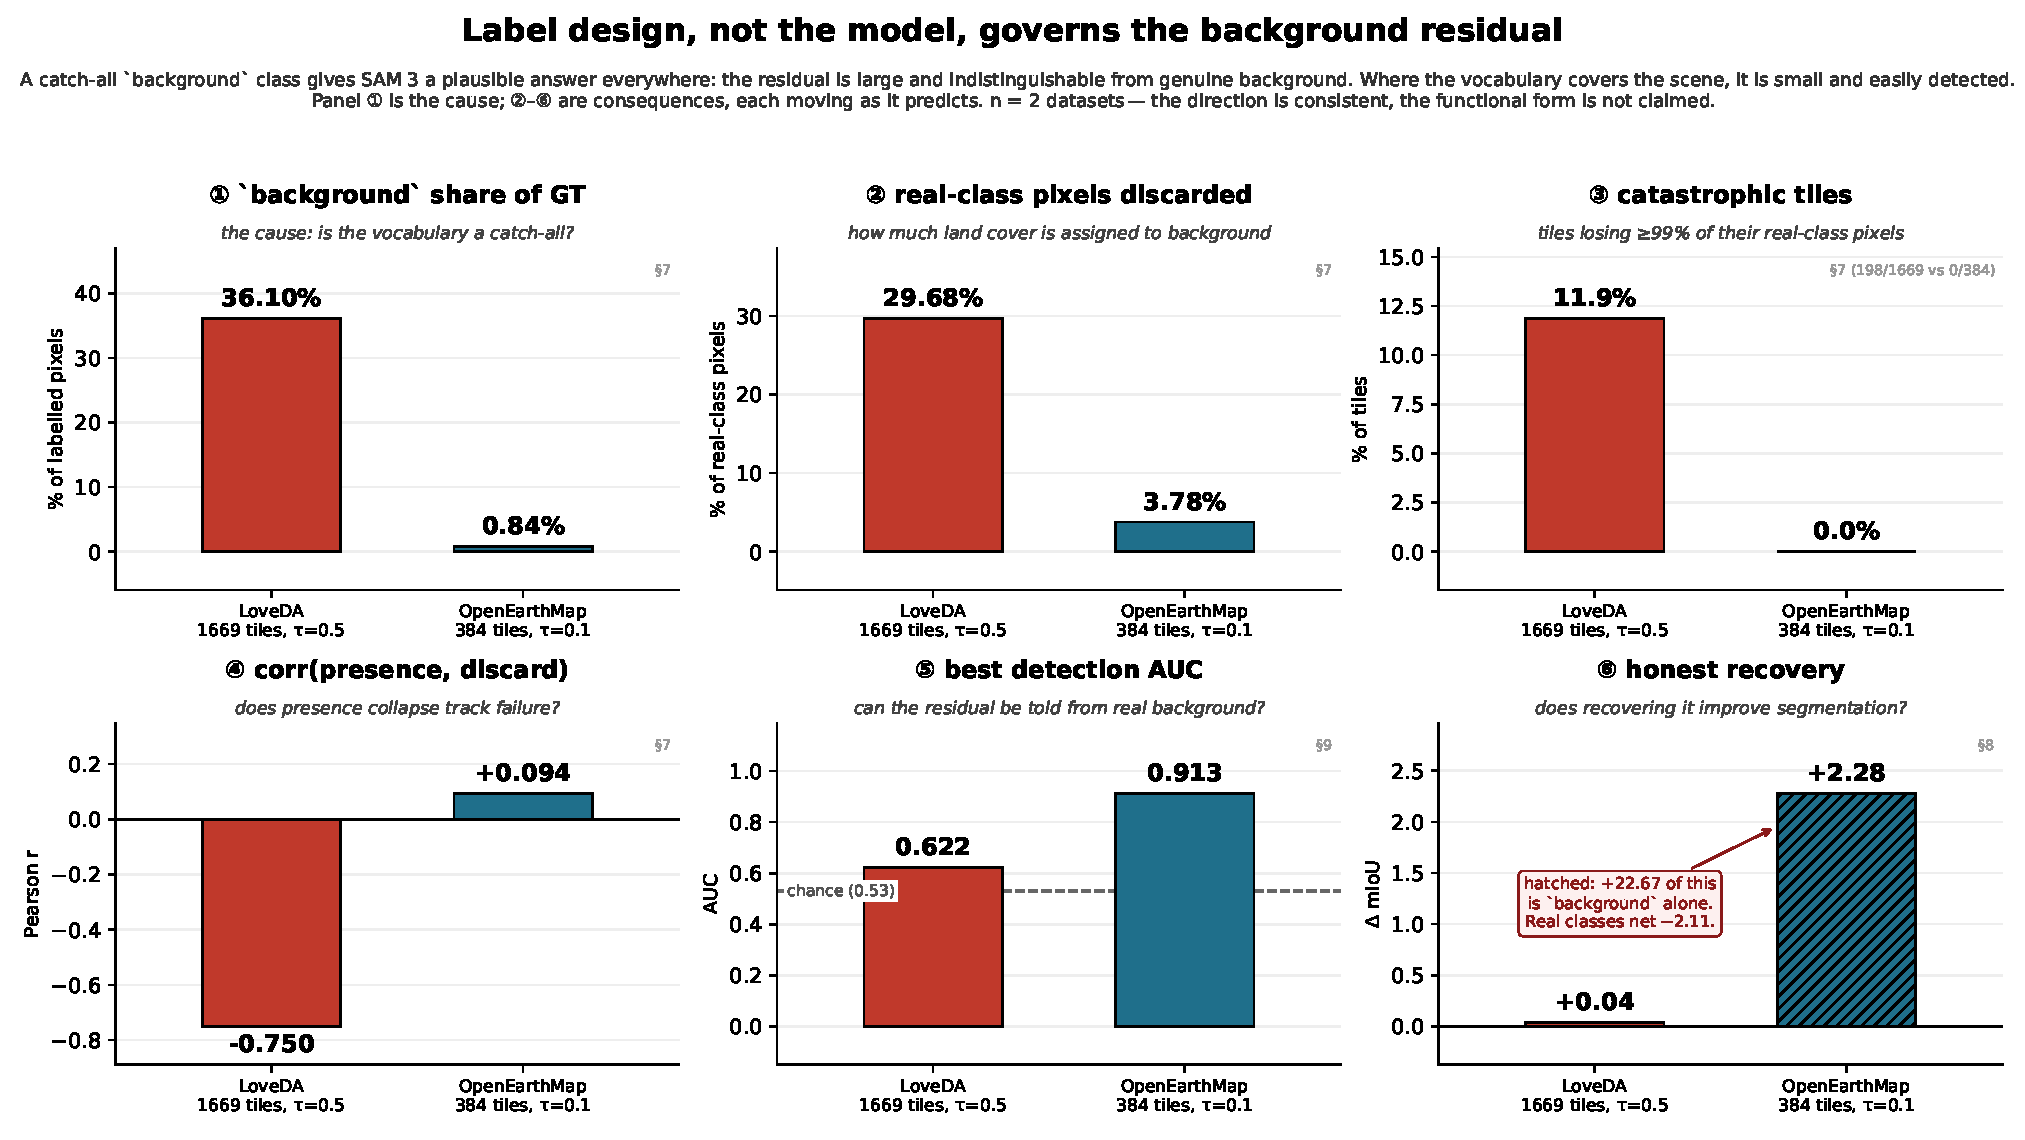
\includegraphics[width=\textwidth]{fig2_mechanism.pdf}
\caption{\todo{caption} Six panels; the catch-all share as the common cause.}
\label{fig:mechanism}
\end{figure*}

\todo{State explicitly that two LoveDA-only claims do \emph{not} generalise:
the presence-collapse correlation (\presCorrLove{} vs \presCorrOEM{}) and the
\discardPct{} headline itself.}

% =====================================================================
\section{What we built, and which parts are justified}
\label{sec:built}
\todo{Region atoms: SLIC, ceiling \ceilSLIC{} against \ceilCC{} for connected
components (Fig.~\ref{fig:purity}). Twenty ceiling points, against \priorOracle{}
for a \emph{perfect} co-occurrence matrix.}

\todo{The prior: boundary marginals, Dirichlet smoothing, directedness via the row
conditional. Signal \pmiSignal{} bits against a \pmiFloor{} permutation floor
(\pmiRatio{}$\times$); mined matrix agrees with ground truth at $\rho=\rhoMined{}$,
and the circularity concern is retired at \rhoCirc{}.}

\subsection{The method: per-class thresholds}
\label{sec:method}
One threshold per class, fitted by coordinate ascent on a calibration subset and
evaluated on disjoint tiles. \emph{No model weights are trained.} SegEarth-OV3
already tunes its single $\tau$ per dataset using labels, so this is the same
protocol with $N$ parameters instead of one.

\todo{Why it works, with \texttt{water} as the case: baseline precision/recall
$89.5/54.7$, so it is right nine times in ten when it fires and finds half of what is
there. Its fitted $\tau$ is \methodWaterTau{} against a global $0.5$, and it gains
\methodWater{} IoU alone. The classes that gain are exactly those with a large
precision--recall asymmetry.}

\todo{The fit maximises land-cover mIoU, \emph{excluding} the catch-all, and say why:
optimising full mIoU lets the search buy the metric by repairing an over-predicted
background. Full mIoU is still what is reported.}

\begin{figure*}[t]\centering
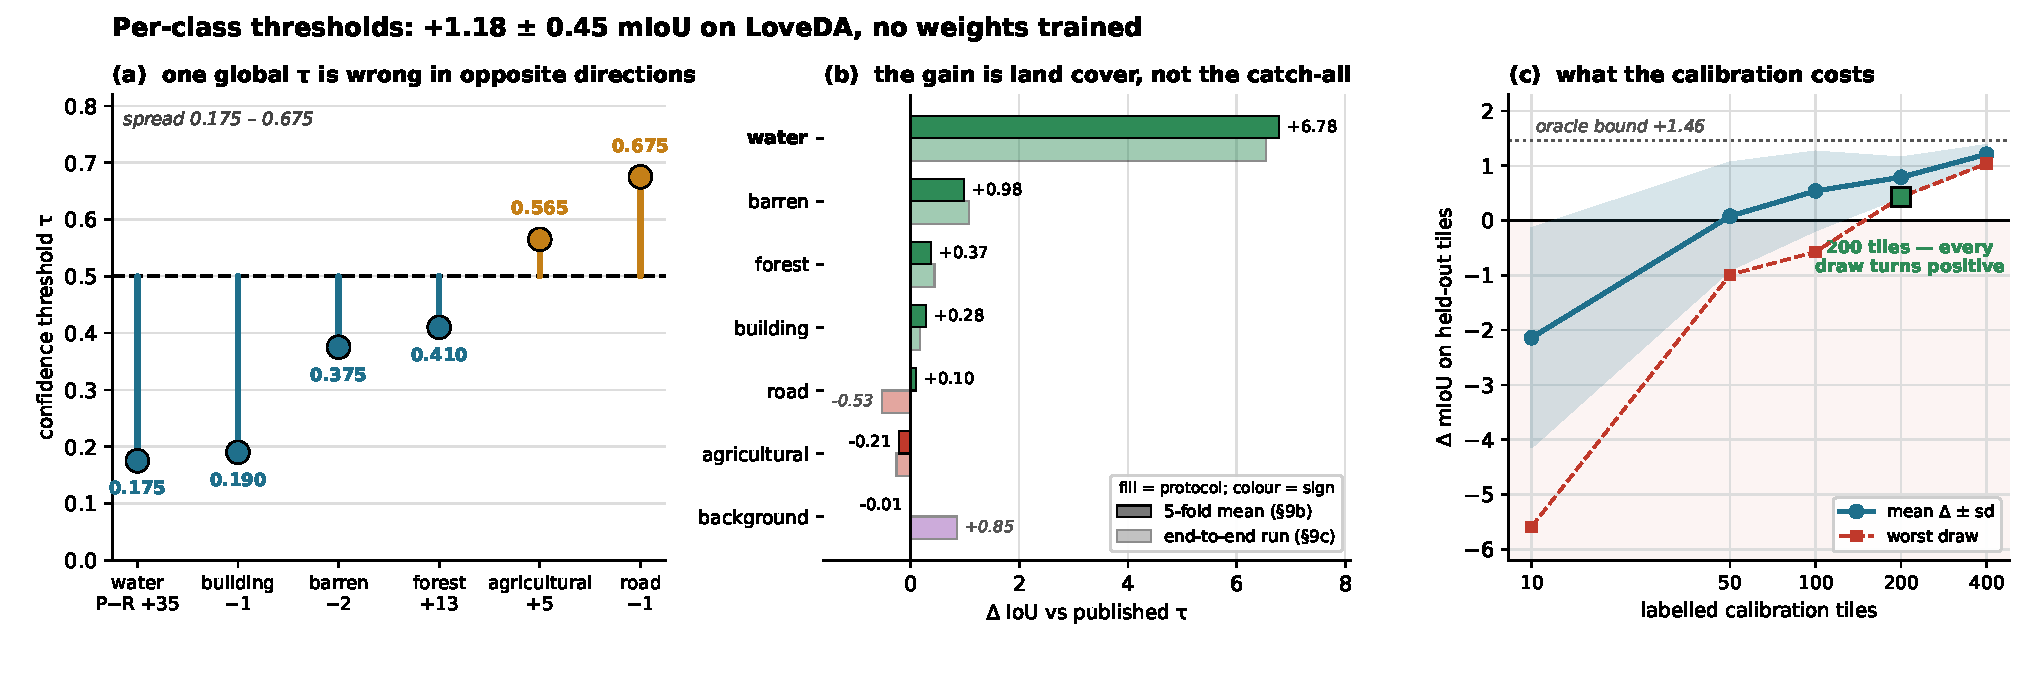
\includegraphics[width=\textwidth]{fig7_method.pdf}
\caption{\todo{caption} (a)~the fitted thresholds span \eeSpread{} against a single
$0.5$; (b)~the gain is land cover, the catch-all is untouched; (c)~\calibTiles{}
labelled tiles is where every draw turns positive.}
\label{fig:method}
\end{figure*}

% =====================================================================
\section{Results}
\label{sec:results}

\begin{table}[t]\centering\small
\caption{The method. Five-fold cross-validation on LoveDA, every fold positive.
The published-$\tau$ baseline is recomputed on the same held-out tiles.}
\label{tab:method}
\begin{tabular}{lrr}
\toprule
 & LoveDA & OpenEarthMap \\
\midrule
$\Delta$ mIoU (5-fold)          & \best{\methodGain{} $\pm$ \methodSD{}} & $+0.16 \pm 0.93$ \\
worst fold                      & \methodWorst{} & --- \\
land-cover classes, aggregate   & \best{\methodLand{}} & \best{$+12.45$} \\
catch-all class                 & \methodBg{}    & $-11.04$ \\
oracle bound                    & \oracleBound{} & --- \\
share of the bound captured     & \oracleShare{} & --- \\
\bottomrule
\end{tabular}
\end{table}

\todo{Beside Table~\ref{tab:method}: OEM's land cover improves substantially while
full mIoU stays flat, because its \texttt{background} sits at 17.13 IoU and pays for
the gain. A caveat about the benchmark, not about the method.}

\paragraph{End-to-end verification.} A single fit on \calibTiles{} calibration tiles,
deployed in the pipeline, moves \eeBase{}~$\to$~\eeFit{} on \eeTiles{} held-out tiles ---
reproducing the cached-histogram prediction exactly, every per-class delta within
$0.04$. \todo{Note honestly that in this single fit \texttt{background} gains $+0.85$
(10\% of the total, incidental --- the objective excludes it) and \texttt{road} loses
$0.53$. A per-class rule can hurt a per-class result.}

\begin{table}[t]\centering\small
\caption{Every intervention we measured, with an oracle bound where one exists.
Each is a trivial alternative a reviewer would otherwise propose.}
\label{tab:interventions}
\begin{tabular}{lrr}
\toprule
intervention & LoveDA & OpenEarthMap \\
\midrule
lower $\tau$ to $0.1$              & \tauCost{} \small(\tauRatio{} wrong per right) & --- \\
remove presence gating             & \presCost{} & --- \\
co-occurrence prior over neighbours& \priorGain{} \small(oracle \priorOracle{}) & --- \\
honest recovery                    & \recoverLove{} & \recoverOEM{}\,$^\dagger$ \\
per-class $\tau$, label-free       & $-0.17$ & $+4.77$\,$^\dagger$ \\
\textbf{per-class $\tau$, calibrated} & \best{\methodGain{}} & $+0.16$ \\
\bottomrule
\end{tabular}
\\[2pt]\footnotesize $^\dagger$ catch-all artefact --- see Table~\ref{tab:oemperclass}.
\end{table}

\begin{table}[t]\centering\small
\caption{\textbf{The honesty of the paper.} OpenEarthMap's headline
\recoverOEM{}~mIoU from recovery is \emph{not} a segmentation improvement.}
\label{tab:oemperclass}
\begin{tabular}{lr}
\toprule
\texttt{background} & \best{\oemBgGain{}} \\
eight real classes, aggregate & \best{\oemRealLoss{}} \\
\texttt{building} (the baseline's best class) & \oemBuildLoss{} \\
\bottomrule
\end{tabular}
\end{table}

\begin{figure}[t]\centering
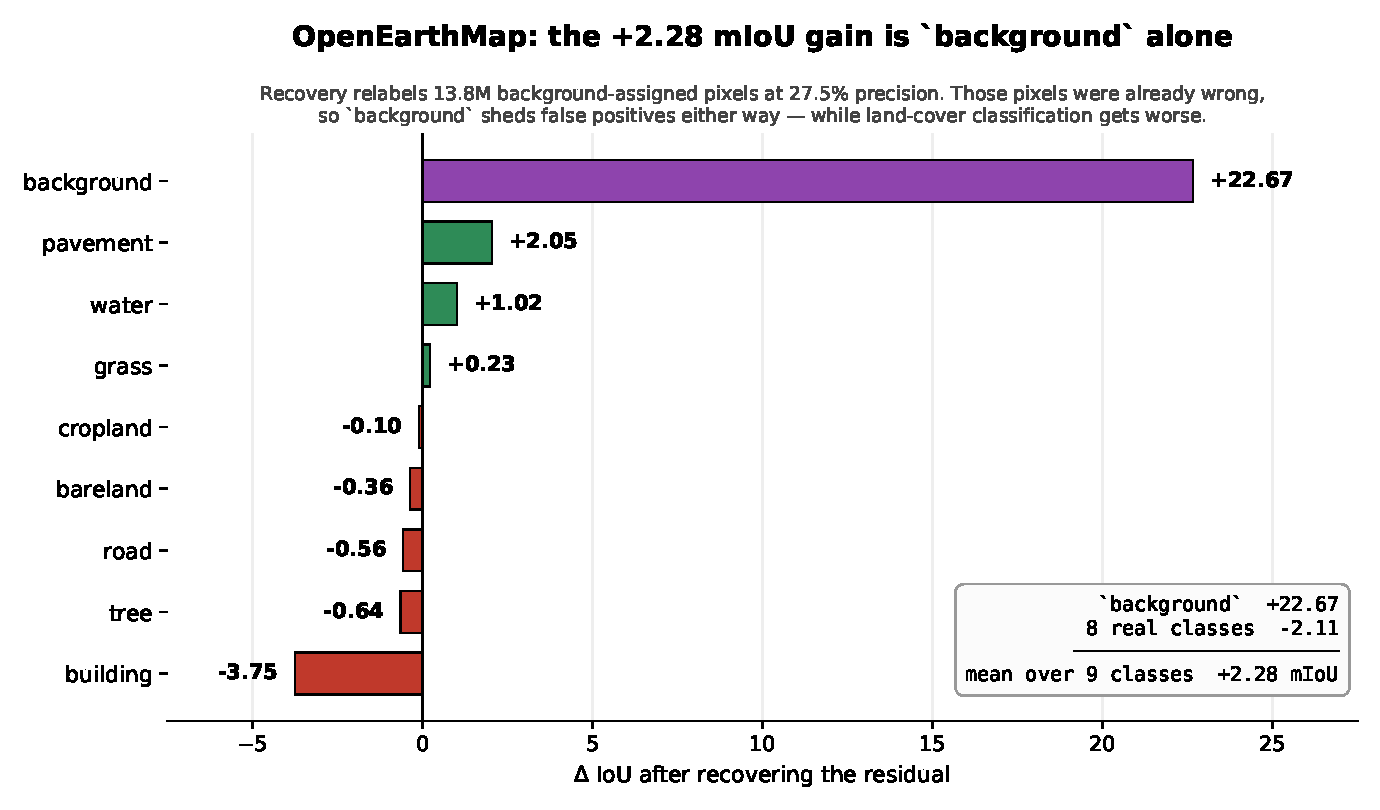
\includegraphics[width=\columnwidth]{fig3_oem_per_class.pdf}
\caption{\todo{caption} Per-class decomposition of OpenEarthMap's \recoverOEM{}.}
\label{fig:oemperclass}
\end{figure}

\begin{figure}[t]\centering
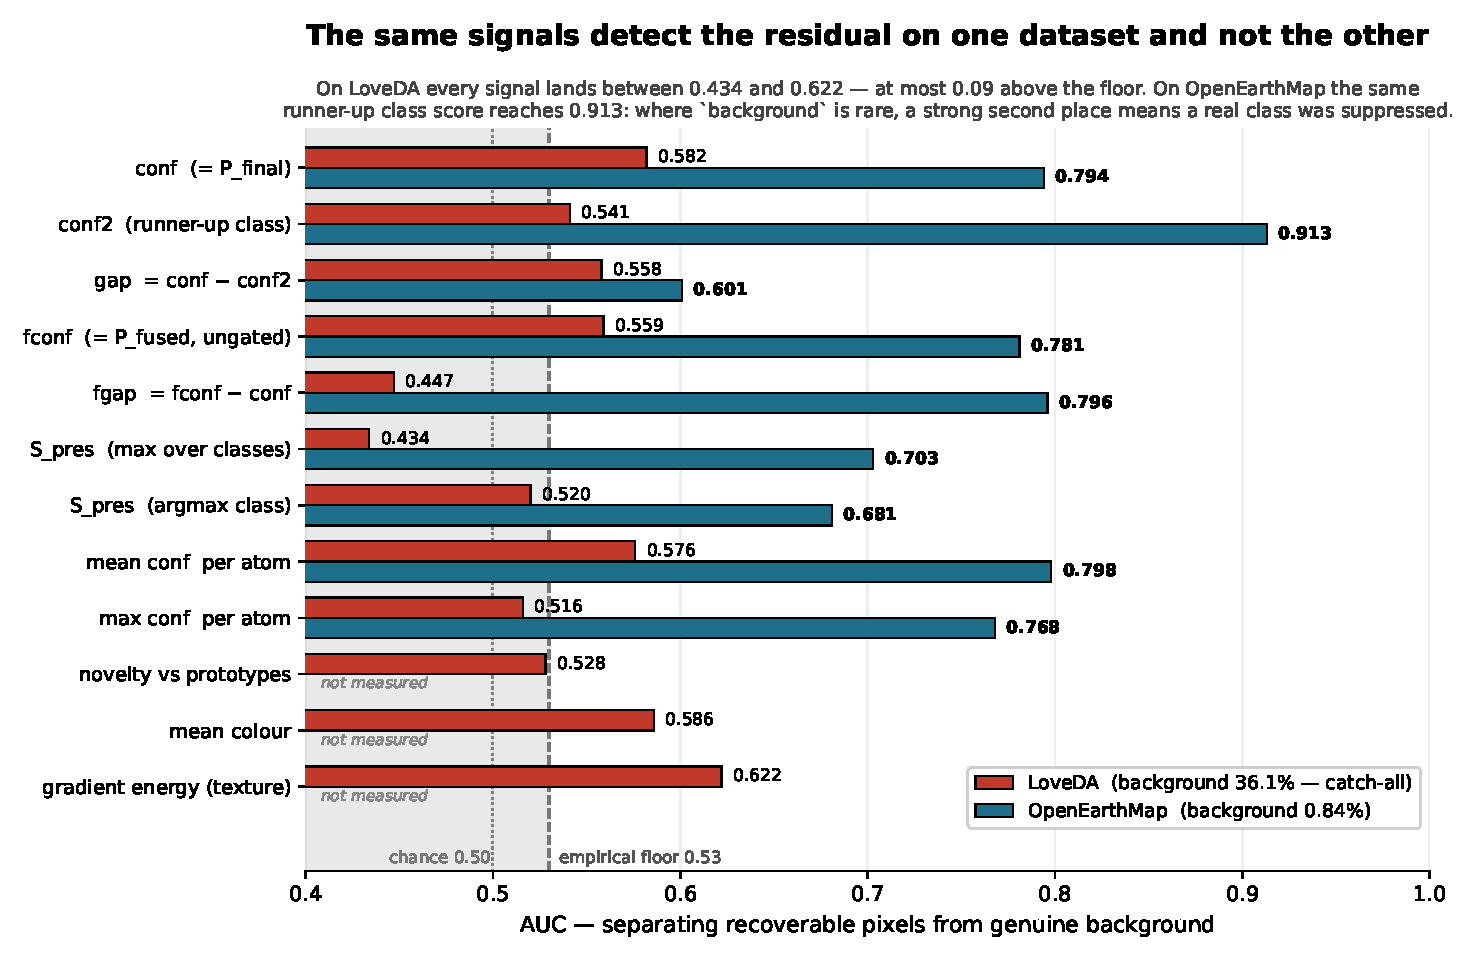
\includegraphics[width=\columnwidth]{fig4_detection_auc.pdf}
\caption{\todo{caption} Nine detection signals, both datasets, against an
empirical floor of \aucFloor{}.}
\label{fig:auc}
\end{figure}

\begin{figure}[t]\centering
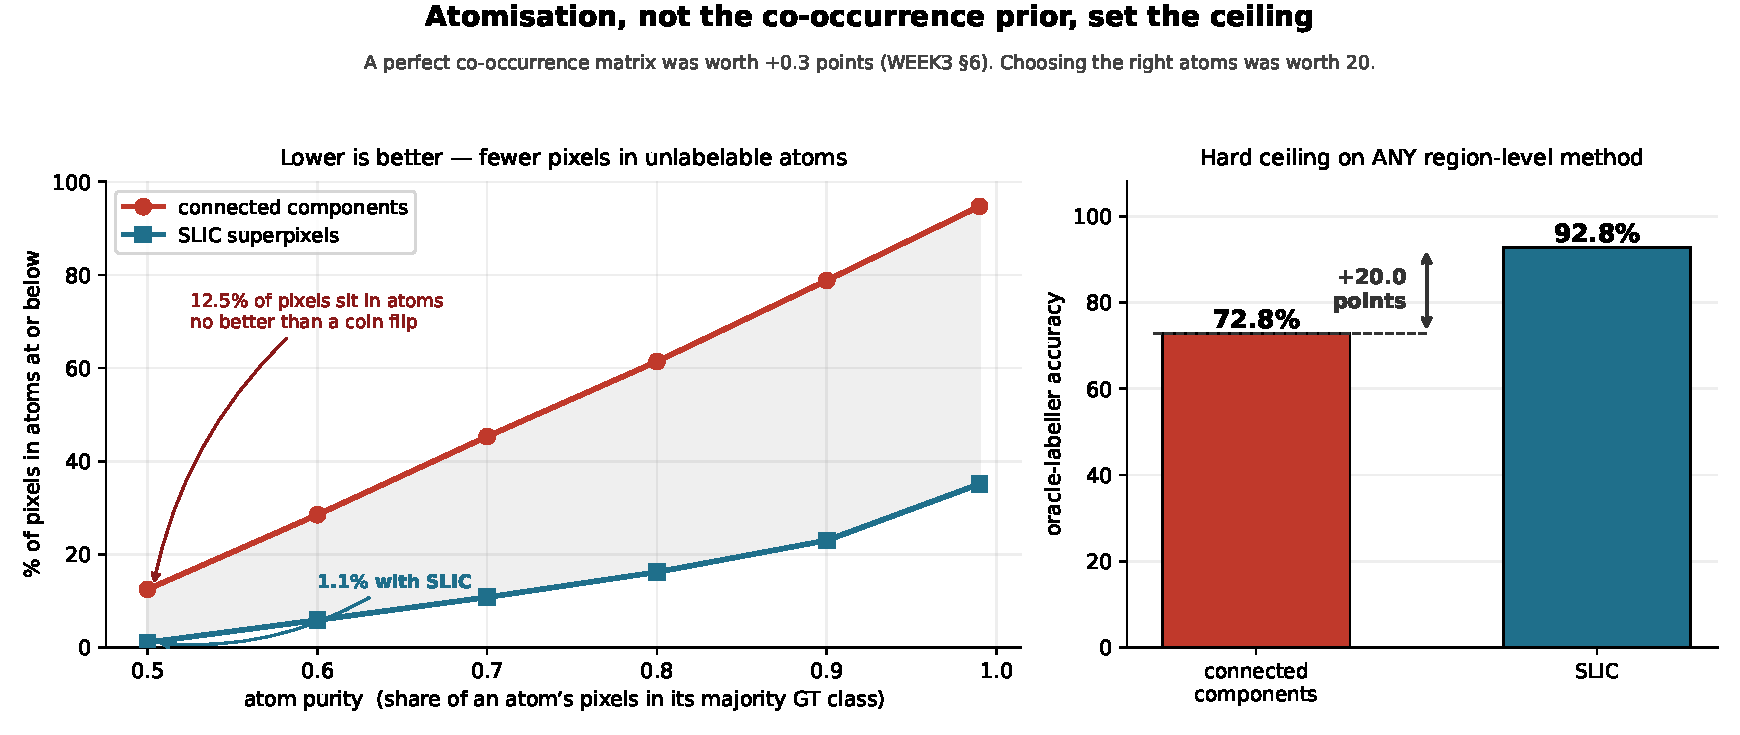
\includegraphics[width=\columnwidth]{fig5_atom_purity.pdf}
\caption{\todo{caption} Atom purity and oracle ceiling, connected components
vs SLIC.}
\label{fig:purity}
\end{figure}

\subsection{The label-free bound, and why it holds}
\label{sec:bound}
The best global $\tau$ is worth \globalOracle{}; the best \emph{per-class} $\tau$ is
worth \oracleBound{}. We tested \nAttempts{} label-free rules and none reaches it;
the best scores \proxyBest{} against a random-proxy control whose 95th percentile is
\proxyCtrl{}.

\paragraph{The reason is not the one we first proposed.} We had supposed the oracle
exploits per-class \emph{precision}, which is label-derived by definition. Precision
is in fact predictable without labels: mean confidence ranks the classes at
$\rho=\proxyConfRho{}$ ($p=\proxyConfP{}$), and agreement between SAM~3's two heads at
$\rho=\proxyHeadRho{}$ ($p=\proxyHeadP{}$), by exact enumeration of all $720$
relabelings. Both move mIoU by less than $0.1$.

\todo{The restated bound, which is the contribution: the optimal per-class threshold
solves a \emph{coupled} multi-class IoU objective --- raising one class's $\tau$ moves
pixels into \texttt{background} and changes every other class's optimum --- so no
per-class scalar can express it, measurable or not. Evidence: precision itself does
not predict the oracle threshold ($\rho=\proxyTauRho{}$, $p=\proxyTauP{}$) and the
relation is not even monotone. This explains why the $N$-parameter fit works and
every one-parameter rule fails.}

% =====================================================================
\section{Limitations}
\label{sec:limitations}
% Write this honestly. PAPER_OUTLINE: it is the section that most reliably
% distinguishes a strong project from a mediocre one.
\begin{itemize}\itemsep2pt
  \item Two datasets, and OpenEarthMap at \oemTiles{}/500 tiles.
  \item \textbf{Calibration must match the evaluation distribution.} Fitting on
        LoveDA \emph{train} and evaluating on val gives \trainToVal{}, because the
        splits differ $2\times$ in discard rate at essentially identical catch-all
        share. \todo{This also constrains the mechanism: share alone cannot be the
        driver.}
  \item Oracle bounds are upper bounds \emph{under our labeller}, not true ceilings.
  \item \todo{The mechanism is confounded at $n=2$: catch-all \emph{share} and
        catch-all \emph{confusability} move together across our two datasets, and the
        second is arguably the more plausible cause. A third dataset that separates
        them is the natural next experiment.}
\end{itemize}

% =====================================================================
\section{Conclusion}
\label{sec:conclusion}
\todo{The residual is a property of the annotation scheme as much as of the model,
and detectability follows the same axis. Neither makes recovery worthwhile. Fixing
the threshold beats recovering the residual --- and the per-class decomposition shows
why a positive mIoU number here would otherwise have been misleading.}

\bibliographystyle{plain}
\bibliography{refs}
\end{document}
